\documentclass{article}
\usepackage[utf8]{inputenc}
\usepackage[T1]{fontenc}
\usepackage{babel}
\usepackage{url}
\usepackage{amssymb,amsmath,amsthm}
\usepackage{hyperref}
\usepackage{listings}
\usepackage{xcolor}
\usepackage{tikz}
\usetikzlibrary{arrows,
                positioning,
                quotes,
                shapes}
\lstset{language=C++,
                frame=tb,
                aboveskip=3mm,
                belowskip=3mm,
                showstringspaces=false,
                columns=flexible,
                basicstyle={\scriptsize\ttfamily},
                numbers=none,
                keywordstyle=\color{blue}\ttfamily,
                stringstyle=\color{red}\ttfamily,
                commentstyle=\color{green}\ttfamily,
                morecomment=[l][\color{magenta}]{\#}
        }
\newcommand{\nodes}[1]{%
    \foreach \num [count=\n starting from 0] in {#1}{
      \node[minimum size=3mm, draw, circle,fill=black!10] (n\n) at (\n,0) {\textbf{\num}};
    }
}
\newtheorem{lemma}{Lemma}
\newtheorem{corollary}{Corollary}
\tikzstyle{arrow} = [thick,->,>=stealth]
\tikzstyle{dashedarrow} = [dashed,->,->=stealth]
\begin{document}
\title{ \textbf{Union Find}}
\author{Niccolò Piazzesi\\n.piazzesi@studenti.unipi.it}
\maketitle
\begin{abstract}
The Union Find data structure, also called Disjoint Set Union (DSU) is a very interesting data structure, not 
only  for the algorithmic techniques and  analysis involved, but also for its applications, especially to graph problems. In this
report I will present a high level view of UnionFind, describing the fundamental structure and the various implementations. In the last section, I will also present
a collection of problems for which the use of a DSU provides an efficient solution.
\end{abstract}
\section{Description}
Suppose we have a collection S of \emph{n} distinct elements, let's say the integers from 1 to \emph{n}. 

Initially these elements
are organized in n disjointed sets \{1\},\{2\},...,\{n\}. For simplicity we will assume that the name of set \{i\}
is i. In the union find problem we want to maintain a collection of disjointed sets while supporting the following operations:
\begin{itemize}
    \item \textbf{union}(A, B): join the sets A and B in a single set $A \cup B$. The old sets A and B are destroyed.
    \item \textbf{find}($x$): given an element $x$, return the name of the set that contains it.
\end{itemize}
Let's now generalize the problem. We have assumed that the n elements are already given. This is not true in general, so we need a way to 
add new elements (and consequentially new sets). This is solved by introducing a third operation:
\begin{itemize}
    \item \textbf{makeSet}($x$): Create a new set {$x$} containing the single element $x$.
\end{itemize}
    We will say that the UnionFind problem consists of maintaining a collection of disjointed sets during 
an arbitrary sequence of \emph{makeSet, union} and \emph{find} operations, starting from the empty set \cite{demetrescu}. Figure \ref{fig:circle} shows a
simple example where the elements considered are numbers.

\begin{figure}
    \centering

    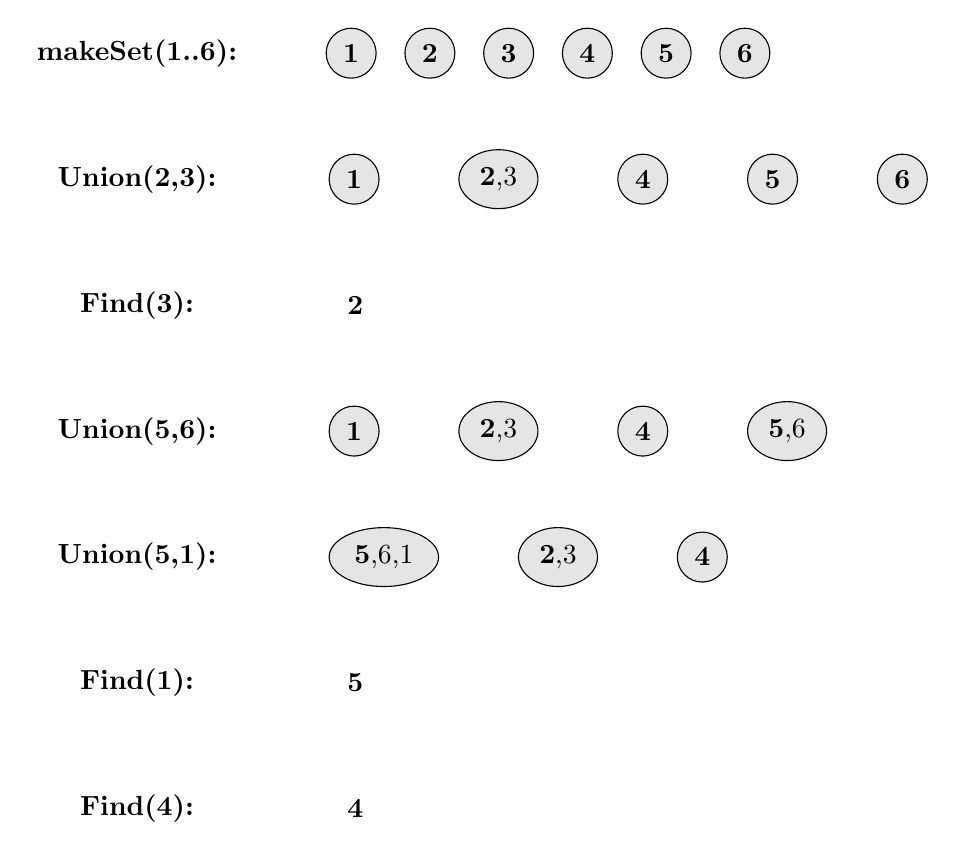
\begin{tikzpicture}
    
    \nodes{1,2,3,4,5,6}
    
    \node[minimum size = 3mm](start)[left=1cm of n0]{\textbf{makeSet(1..6):}};
    \node[minimum size=3mm] (u1)[below=of start] {\textbf{Union(2,3):}};
    \node[circle,fill=black!10, draw, minimum size=3mm] (u1n1)[right=1.3cm of u1] {\textbf{1}};
    \node[ellipse,fill=black!10,draw,fill=black!10, minimum size=3mm] (u1n2)[right=1cm of u1n1] {\textbf{2},3};
    \node[circle,fill=black!10, draw, minimum size=3mm] (u1n3)[right=1cm of u1n2] {\textbf{4}};
    \node[circle,fill=black!10, draw, minimum size=3mm] (u1n4)[right=1cm of u1n3] {\textbf{5}};
    \node[circle,fill=black!10, draw, minimum size=3mm] (u1n5)[right=1cm of u1n4] {\textbf{6}};
    
    \node[minimum size=3mm] (f1) [below= of u1]{\textbf{Find(3):}};
    \node[minimum size=3mm] (f1n1)[right=1.7cm of f1]{\textbf{2}};
    
    \node[minimum size=3mm] (u2)[below=of f1] {\textbf{Union(5,6):}};
    \node[circle,fill=black!10, draw, minimum size=3mm] (u2n1)[right=1.3cm of u2] {\textbf{1}};
    \node[ellipse,fill=black!10,draw, minimum size=3mm] (u2n2)[right=1cm of u2n1] {\textbf{2},3};
    \node[circle,fill=black!10, draw, minimum size=3mm] (u2n3)[right=1cm of u2n2] {\textbf{4}};
    \node[ellipse,fill=black!10,draw, minimum size=3mm] (u2n4)[right=1cm of u2n3] {\textbf{5},6};
    
    \node[minimum size=3mm] (u3)[below=of u2] {\textbf{Union(5,1):}};
    \node[ellipse,fill=black!10,draw, minimum size=3mm] (u3n1)[right=1.3cm of u3] {\textbf{5},6,1};
    \node[ellipse,fill=black!10,draw, minimum size=3mm] (u3n2)[right=1cm of u3n1] {\textbf{2},3};    
    \node[circle,fill=black!10, draw, minimum size=3mm] (u3n3)[right=1cm of u3n2] {\textbf{4}};
    
    \node[minimum size=3mm] (f2) [below= of u3]{\textbf{Find(1):}};
    \node[minimum size=3mm] (f2n1)[right=1.7cm of f2]{\textbf{5}};

    \node[minimum size=3mm] (f3) [below= of f2]{\textbf{Find(4):}};
    \node[minimum size=3mm] (f3n1)[right=1.7cm of f3]{\textbf{4}};
    
    \draw [arrow] (u2) (u2n1);
    \end{tikzpicture}
    
    \caption{A running example with 6 initial elements. The name of each set is written in bold}
    \label{fig:circle}
\end{figure}

\section{Naive Implementations}
The general idea for implementing UnionFind is to represent the collection as a forest of trees, with each tree representing a single set. 
In the following code we will  consider integers as elements and use an array representation of the forest.
Given an array \emph{parents} the element \emph{parents[i]} contains the father of element \emph{i} in the tree hierarchy. For the root
r of a tree we will have parents[r] $=$ r. Before analyzing a more efficient implementation, we will see two simpler versions.

\subsection{QuickFind} \label{QF}
QuickFind aims at having a very good time complexity for the find operation. To achieve this, it represent each set as a tree of height 1. Each element
has a pointer to the root of the tree,  and the root contains the name of the set. The find operation simply follows the pointer and returns the root. It's easy to see that it has $O(1)$ time complexity. MakeSet(e) creates a new tree composed by two nodes: the root and a single leaf child. It stores e in both of them. MakeSet is $O(1)$ as well. The union operation deletes the pointer from the elements to the root of the old tree
and add new pointers to the root of the new tree. In the worst case, this takes $O(n)$. Space complexity is $O(n)$. 

\begin{figure}[h!]
    \centering
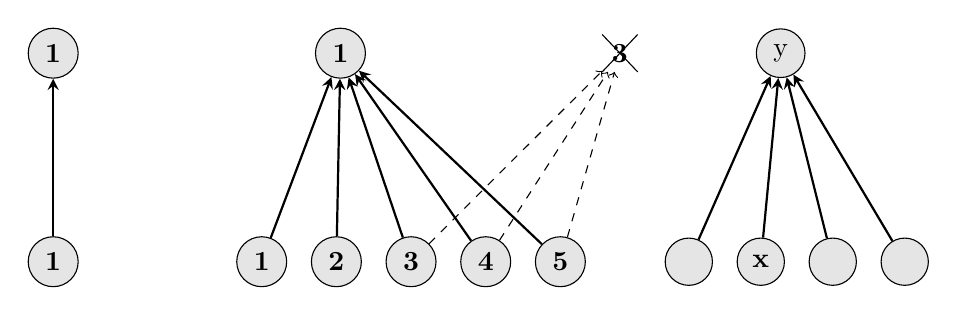
\begin{tikzpicture}
 
    
    \node[circle,fill=black!10, draw=, minimum size=3mm] (qf8) at (0,0) {\textbf{1}};
    \node[circle,fill=black!10, draw=, minimum size=3mm] (qf9) [below = 2cm of qf8] {\textbf{1}};
    \node[circle,fill=black!10, draw=, minimum size=3mm] (qf1)[right= 3cm of qf8] {\textbf{1}};
    \node[circle,cross out, draw, minimum size=3mm] (qf2)[right= 3cm of qf1] {\textbf{3}};
    \node[circle,fill=black!10, draw, minimum size=3mm] (qf3)[right= 2cm of qf9] {\textbf{1}};
    \node[circle,fill=black!10, draw, minimum size=3mm] (qf4)[right= 0.3cm of qf3] {\textbf{2}};
    \node[circle,fill=black!10, draw, minimum size=3mm] (qf5)[right= 0.3cm of qf4] {\textbf{3}};
    \node[circle,fill=black!10, draw, minimum size=3mm] (qf6)[right= 0.3cm of qf5] {\textbf{4}};
    \node[circle,fill=black!10, draw, minimum size=3mm] (qf7)[right= 0.3cm of qf6] {\textbf{5}};
    
    \node[circle,fill=black!10, draw=, minimum size=6mm] (qf10) [right = 1.5cm of qf2] {y};
    \node[circle,fill=black!10, draw=, minimum size=6mm] (qf11) [right = 1cm of qf7] {};
    \node[circle,fill=black!10, draw=, minimum size=6mm] (qf12) [right = 0.3cm of qf11] {\textbf{x}};
    \node[circle,fill=black!10, draw=, minimum size=6mm] (qf13) [right = 0.3cm of qf12] {};
    \node[circle,fill=black!10, draw=, minimum size=6mm] (qf14) [right = 0.3cm of qf13] {};
    \draw [arrow] (qf3) -- (qf1);
    \draw [arrow] (qf4) --(qf1);
    \draw [arrow] (qf5) --(qf1);
    \draw [arrow] (qf6) --(qf1);
    \draw [arrow] (qf7) --(qf1);
    \draw [arrow] (qf9) --(qf8);
    \draw [arrow] (qf11) -- (qf10);
    \draw [arrow] (qf12) -- (qf10);
    \draw [arrow] (qf13) -- (qf10);
    \draw [arrow] (qf14) -- (qf10);
    \draw [dashedarrow] (qf5) -- (qf2);
    \draw [dashedarrow] (qf6) -- (qf2);
    \draw [dashedarrow] (qf7) -- (qf2);
\end{tikzpicture}
\caption{makeSet(1), Union(1, 3) and find(x) = y using QuickFind}

\label{fig:quickFind}
\end{figure}
Listing \ref{lab:qf} shows a possible implementation in $C++$. As i said before,
we use an array representation so each pointer becomes simply an element of the array.
If  we want to compute find(i) we return the element parents$[i]$;
\begin{center}
    \lstinputlisting[language=C++,caption=Quickfind implementation,label=lab:qf]{code/quickFind.cpp} 
\end{center}

\subsection{QuickUnion} \label{QU}
In QuickUnion we also use trees, but they can have height $\neq$ 1. Each element has a pointer to their
father. MakeSet(x) creates a single node named x. Union(A,B) makes the root of B a child of the 
root of A. The find operation is slightly more complex. Let's say
we want to compute find(\emph{e}) for a generic \emph{e}. Starting from \emph{e} we repeatedly 
follow the pointer to the father until we find the root of the tree.
\begin{figure}[h!]
    \centering
    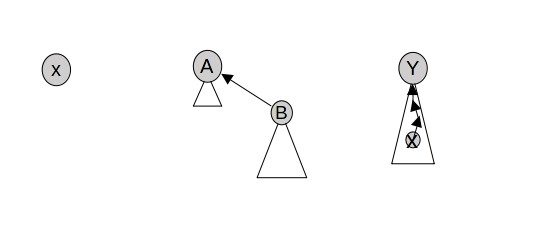
\includegraphics[width=0.8\textwidth]  {img/uf.jpg}
    \caption{makeSet(x), union(A,B) and find(x) = y in QuickUnion}
    \label{fig:quickUnion}
\end{figure}

The time complexity of find grows linearly with the height of the tree. It's easy to see
that, if we start with $n$ disjointed sets the worst case is having a tree of height $n$. A sequence
of $n-1$ union operations that could lead to this case is the following: union(1,2), union(2,3),..., union(n-1,n).
In this situation, find has $O(n)$ time complexity. 
\begin{center}
    \lstinputlisting[language=C++,caption=QuickUnion implementation,label=lab:qu]{code/quickUnion.cpp} 
\end{center}
Let's discuss the cost of union. As previously said,
this consists in creating a new pointer from the root of the old tree to the root of the new tree. This can be done 
very easily in $O(1)$ time. If we look at the implementation in Listing \ref{lab:qu}, we notice
that in the union operation we first call find to find the root of the trees containing the elements. Find takes $O(n)$ and this dominates the 
total complexity, so the union method in that code takes $ O(n)$ as well. But this is just one possible implementation. We are analyzing
the abstract operation, so our previous analysis is still valid. 

\section{Balancing Heuristics}
Now we will see some heuristics that aim to improve the time complexity of union find. In particular,
we will first see a heuristic to improve union in the quickFind algorithm, and then various heuristics to improve
find in the QuickUnion algorithm. Note that in this section we will simply describe the techniques, while the 
complexity analysis will be shown in the next part.
\subsection{Balancing union in QuickFind}
To improve the performance of QuickFind we must focus on the most expensive operation, which we know is 
union. We can observe that the implementation that we described in section \ref{QF} is not very smart. The more $ | B | $ grows the more
Union(A, B) costs. When we have $|A| < |B| $ it is more efficient to move the nodes of the set A.

\begin{figure}[h!]
    \centering
    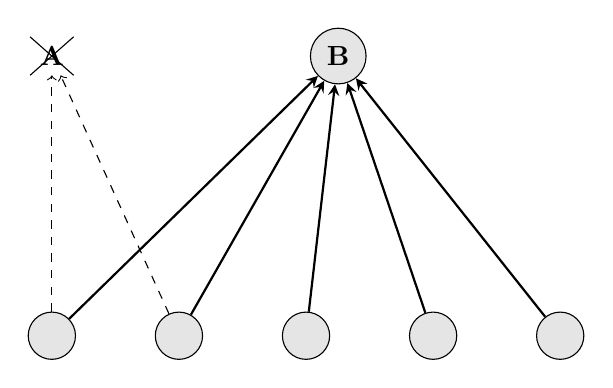
\begin{tikzpicture}
        
        \node[circle,cross out,fill=black!10, draw=, minimum size=3mm] (qf1) at (0,0) {\textbf{A}};
        \node[circle,fill=black!10, draw=, minimum size=6mm] (qf2)[right= 3cm of qf1] {\textbf{B}};
        \node[circle,fill=black!10, draw=, minimum size=6mm] (qf3)[below= 3cm of qf1] {};
        \node[circle,fill=black!10, draw=, minimum size=6mm] (qf4)[right= 1cm of qf3] {};
        \node[circle,fill=black!10, draw=, minimum size=6mm] (qf5)[right= 1cm of qf4] {};
        \node[circle,fill=black!10, draw=, minimum size=6mm] (qf6)[right= 1cm of qf5] {};
        \node[circle,fill=black!10, draw=, minimum size=6mm] (qf7)[right= 1cm of qf6] {};
        \draw[dashedarrow] (qf3) -- (qf1);
        \draw[dashedarrow] (qf4) -- (qf1);
        \draw[arrow] (qf3) -- (qf2);
        \draw[arrow] (qf4) -- (qf2);
        \draw[arrow] (qf5) -- (qf2);
        \draw[arrow] (qf6) -- (qf2);
        \draw[arrow] (qf7) -- (qf2);
    \end{tikzpicture}
    \caption{Union(A,B) when $|A| < |B|$}
    \label{fig:qfsize}
\end{figure}
In the implementation, we store an auxiliary array \emph{size}, which keeps track
of the cardinality of each set.

\begin{lstlisting}[caption=updated operations in QuickFind, label=lab:qfu]
    QuickFind(int n) : n(n){
        parents.resize(n);
        std::iota(parents.begin(), parents.end(), 0);
        std::vector<int> size(n, 1);
    }

    void makeSet(int x){
        if (x >= parents.size())
            parents.resize(x);
        parents.at(x) = x;
        size.at(x) = 1;
    }
    void set_union(int a, int b)
    {
        if (a != b){
            if(size[a] < size[b]) std::swap(a,b);
            for (auto i : parents){
                if (i == b)
                    i = a;
            }
            size[a] += size[b];
        }
    }
    
\end{lstlisting}
\subsection{Balancing heuristics for QuickUnion}
To improve the QuickUnion algorithm, we need to make \emph{find} more efficient.
In section \ref{QU} we observed that this operation has a worst-case $O(n)$ time complexity.
This is due to the fact that we allow the height of the trees to grow without any control when 
doing a \emph{union}. 
\paragraph{Union by Size}
The first heuristic uses the same idea of the QuickFind union heuristic. When doing \emph{Union(A,B)}
we make the smaller set in size child of the bigger set.
\begin{lstlisting}[caption=Union by size implementation, label=quu]
    void set_union(int a, int b){
        a = find(a);
        b = find(b);
        if (a != b) {
            if (size[a] < size[b])
                std::swap(a, b);
            parents[b] = a;
            size[a] += size[b];
        }
    }

\end{lstlisting}
\paragraph{Union By Rank} In union by rank we use the height of the tree instead
of its size. The approach is the same of Union By size: we attach the shorter tree
to the taller one. It's important to notice that, when we use compression techniques that we will discuss later, the rank is not always equal to the actual height of a tree. 
In this case it gives an upper bound of the height.  
\begin{figure}[h!]
    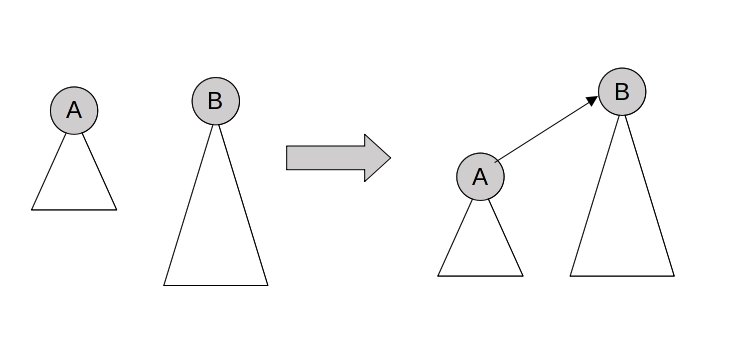
\includegraphics[width=0.9\linewidth]{img/urank.png}
    \caption{Union(A,B) when rank(A) < rank(B)}
    \label{fig:urank}
\end{figure}
\begin{lstlisting}[caption=QuickUnion using Union by Rank]
    QuickUnion(int n) : n(n){
        parents.resize(n);
        std::iota(parents.begin(), parents.end(), 0);
        ranks.resize(n);
    }

    void makeSet(int x){
        if (x >= parents.size())
            parents.resize(x);
        parents.at(x) = x;
        ranks.at(x) = 0;
    }
    void set_union(int a, int b){
        a = find(a);
        b = find(b);
        if (a != b){
            if (ranks[a] < ranks[b])
                std::swap(a, b);
            parents[b] = a;
            if (ranks[a] == ranks[b])
                ranks[a]++;
        }
    }
\end{lstlisting}
To further improve QuickUnion performance, we can also modify \emph{find} in order to reduce the height of a tree
even more. Let $u_0. u_1, \dots, u_{l-1}$ be the nodes visited during \emph{find(x)}, where $u_0 = x$ and $u_{l-1}$ is
the root of the tree containing $x$. We can assume $l \geq 3$, because if $l\leq 2$ we don't need to reduce the height.
We can apply one of the following compression heuristics:
\paragraph{Path compression}  make all the nodes $u_i$ ($ 0 \leq i \leq l-3$) children of the root $u_{l-1}$\cite{hopcroft1973set}.
\begin{lstlisting}
    int find(int x){
        int p = x;
        if (parents[p] != p)
            parents[p] = find(parents[p]); //path compression
        return parents[p];
    }
\end{lstlisting}
\paragraph{Path splitting}  make the node $u_i (0 \leq i \leq l-3)$ a child of its grandparent $u_{i+2}$\cite{van1977alternative} \cite{van1980datastructures}. 
\begin{lstlisting}
    public int find(int x) {
        while (x != parent[x]) {
            int next = parent[x];
            parent[x] = parent[next];   // path splitting
            x = next;
        }
        return x;
    }
\end{lstlisting}
\paragraph{Path halving}  make the node $u_{2i} ( 0 \leq i \leq \lfloor \frac{l-1}{2}\rfloor - 1)$ a child 
of its grandparent $u_{2i+2}$\cite{van1977alternative} \cite{van1980datastructures}.
\begin{lstlisting}
    public int find(int x) {
        while (x != parent[x]) {
            parent[x] = parent[parent[x]];    // path  halving
            x = parent[x];
        }
        return x;
    }
\end{lstlisting}
\begin{figure}[h!]
    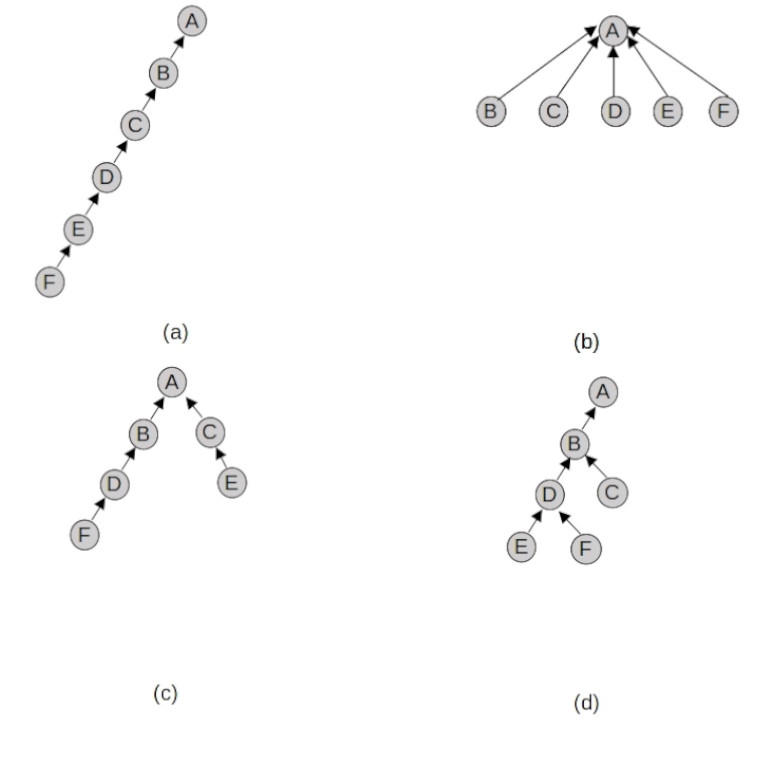
\includegraphics[width = \linewidth]{img/pc.jpg}
    \caption{(a) The tree before executing \emph{find(F)};
    (b) \emph{find(F)} with path compression;
    (c) \emph{find(F)} with path splitting;
    (d) \emph{find(F)} with path halving;
    }
    \label{fig:pc}   
\end{figure}
\newpage
\section{Complexity analysis}\label{complex}
Let's analyze how much the heuristics improve the total time complexity. Note that any combination of 
the union and find heuristics  shown gives the same improvement in terms of time complexity. 

In particular, we will now see
how much does union by rank improves the time complexity of find in the QuickUnion version.
For simplicity, we will not consider any compression heuristic on the find itself for now. 
Let's start with the following result:
\begin{lemma}\label{rank}
    A QuickUnion tree balanced by rank has at least $2^{rank(x)}$ nodes, where $x$ is the root of the tree.
\end{lemma}
\paragraph{\textbf{Proof.}} We demonstrate the lemma by induction on the number of operations. The base case is trivially proven
since we have no trees. Now let's assume that the lemma is valid before an operation and we want to prove that it holds afterwards. When we execute  a find, the rank is not modified and so the lemma still holds.
If we execute a makeSet($x$) we introduce a new tree with the single node $x$, and rank($x$) $ = 0$.
This tree has $2^{rank(x)} = 2^0 = 1$ node  and the lemma is verified. We now consider $union(x, y)$.
We indicate with $|x|$ and $|y|$ the size of the trees before merging them, while $|x \cup y|$ is the size of the resulting tree. Since the two sets are disjointed,
$|x \cup y|$ = $|x| + |y|$.
We have three separate cases:\begin{enumerate}
    \item If $rank(y) < rank(x)$, the root of $y$ becomes a child of the root of $x$. The root of the new tree will have $rank(x \cup y)$ = rank($x$). 
    By inductive hypothesis we have $|x| \geq 2^{rank(x)}\text{ and }|y| \geq 2^{rank(y)}$ and the number
    of nodes in the resulting tree is:
    $$ |x\cup y| = |x| + |y| \geq 2^{rank(x)} + 2^{rank(y)} > 2^{rank(x)} = 2^{rank(x \cup y)} $$
    \item If $rank(y) < rank(x)$, we follow the same reasoning of the first case. The only difference is that
    the root of $x$ becomes a child of the root of $y$.
    $$ |x\cup y| = |x| + |y| \geq 2^{rank(x)} + 2^{rank(y)} > 2^{rank(y)} = 2^{rank(x \cup y)} $$
    \item When $rank(x) = rank(y)$, the union makes the root of $y$ child of the root of $x$ and updates $rank(x)$ to $rank(x) + 1$. This is also the value of $rank(x\cup y)$.
    By using the inductive hypotheses, the number of nodes in new tree is:
    $$  |x\cup y| = |x| + |y| \geq 2^{rank(x)} + 2^{rank(y)} \geq 2\cdot2^{rank(x)} = 2^{rank(x) + 1} = 2^{rank(x \cup y)} $$
\end{enumerate}
In each case the lemma is still true after a union. The following corollary is an immediate consequence.
\begin{corollary}
    During a sequence of makeSet, union and find, the height of a balanced QuickUnion tree has a $\lfloor \log_2 n \rfloor$ upper bound, where $n$
    is the total number of makeSet.
\end{corollary}
\paragraph{Proof.} Let T be a balanced QuickUnion tree, and let $x$ be its root. We call $size(x)$
the number of nodes in T. By definition, the height of T is $rank(x)$ and $size(x) \leq n$. For Lemma
\ref{rank}, we have $size(x) \geq 2^{rank(x)}$ and, if we combine all these results:
$$rank(x) \leq \lfloor \log_2 (size(x))\rfloor \leq \lfloor log_2 n \rfloor.$$

\bigskip

This corollary guarantees that, using union by rank, a QuickUnion tree will have $O(\log n)$ height. As we know, the time complexity of find
is related to the height of the tree and so we can affirm the following result.

\bigskip

\emph{QuickUnion trees balanced by height support makeSet and union operations in constant time. A find takes $O(\log n)$
in the worst case, where $n$ is the total numbers of makeSet executed.}

During any sequence of the operations described, the following properties are verified:
\paragraph{Property 1.} The rank of a generic node $x$ is initially 0 and increases until x remains a root. As soon as x is not root anymore, its rank
remains unchanged.
\paragraph{Property 2.} Let $x$ be a generic, non root node and let $p(x)$ be its father node.
$$rank(p(x)) > rank(x)$$ 
\paragraph{Property 3.} For each node $x$ $ rank(x) \leq \lfloor \log_2 n \rfloor$, where $n$ is the total number of nodes.

\bigskip

In the previous analysis, we did not  consider any compression heuristic during a find. We can use one of them to improve the time complexity
even more. 
Assume that we use Union By Rank combined with path compression.
In 1973, Hopcroft and Ullman proved that a sequence of $m$ makeSet, find or  union is done in $O(m\log^* n)$ time, where $log^*$ is the iterated
logarithm and $n$ the number of makeSet executed \cite{hopcroft1973set}. In 1975, Tarjan proved that the same sequence of operations
is done in $O(m\alpha(n))$ where $\alpha$ is the inverse of the Ackermann function \cite{tarjan1975efficiency}. This function grows even slower than $\log^*$( ).
The proof of this bound is very complex and goes beyond the scope of this report, so it is omitted.  
\section{Applications}
Let's now see some problems where the DSU data structure shows its power.
\subsection{Detect cycle in a graph} \label{loop}
\emph{Given an undirected graph $G = (V, E)$, check if it contains a cycle}
\begin{figure}[h!]
    \centering
    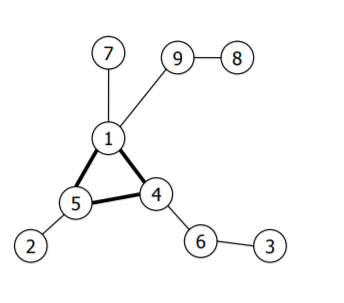
\includegraphics[scale=0.5]{img/cycle.png}
    \caption{A graph with a cycle}
\end{figure}
\bigskip

A trivial solution simply traverse the graph with a DFS visit in $O(|V| + |E|)$
time and space. We can achieve a more space efficient solution using UnionFind. Create a set for each
vertex $v \in V$. Now, for every edge $ (u,v) \in E$:\begin{enumerate}
    \item Find the root  of the sets that contain u and v
    \item If we find  the same root, a cycle has been found and we stop 
    \item Otherwise, merge the two sets
\end{enumerate}

\paragraph{Time complexity.} We do $O(|V| + |E|)$ makeSet, find and union operations.
Thanks  to the results shown in section \ref{complex} we know that this takes $O((|V| + |E|)\alpha(|V|))$ time. 
This is not exactly linear as the trivial solution, but $\alpha$ grows so slowly that, in practice, there is almost no difference in the runtime.

\paragraph{Space complexity.} We do not need to store the visited edges so the space used is only $O(|V|)$.
\lstinputlisting[caption=Cycle detection]{code/graphcycle.cpp}
\subsection{Kruskal's algorithm}
\emph{Given a connected, undirected  and weighted  graph $G = (V,E)$,
find  the \textbf{minimum spanning tree}(MST) of G. The minimum spanning tree 
is a subtree of $G$ that contains all the vertices $v \in V$, and with the minimum possible total edge weight.}
    
\bigskip
\begin{figure}[h!]
    \centering
    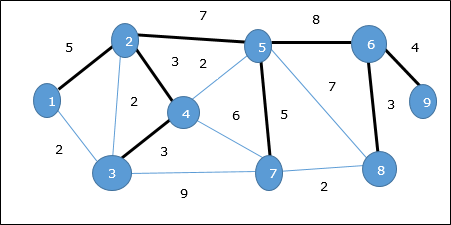
\includegraphics[scale=0.8]{img/mst.png}
    \caption{An example of a minimum spanning tree}
\end{figure}
There are many algorithms to find the MST of a given graph \cite{prim1957shortest} \cite{nevsetvril2001otakar},
but now we will see the algorithm described by Joseph Kruskal \cite{kruskal1956shortest}.
This algorithm starts from an empty tree, and increasingly builds    the MST with the following steps:
\begin{enumerate}
    \item Sort all the edges by increasing weight.
    \item \label{p}Pick the next smallest edge. If it forms a cycle with the  tree formed so far discard the edge, otherwise
    add it to the tree.
    \item Repeat step 2 until there are $|V| - 1$ edges in the tree.
\end{enumerate}
The central point of the algorithm is the cycle detection in step \ref{p}. We can use a modified version of the algorithm described in \ref{loop}.
Given a edge $(u,v)$ we find the sets to which $u$ and $v$ belong. If they are not in the same set, they do not form a cycle 
and so we  add the edge to the current tree and merge the sets together. 
\paragraph{Time complexity.} Sorting the edges is $O(|E|\log|E|)$. Finding cycles takes
$O((|V| + |E|)\alpha(|V|))$. Assuming that the graph is connected, we have

 $$|E| \geq |V| - 1$$, which means that the disjoint sets operations take $O(|E|\alpha(|V|))$. We know that
 $\alpha(|V|) = O(\log|V|)$, and this tells us that the total time complexity of Kruskal's algorithm
 is $O(|E|\log|E|)$ \cite{cormen2009introduction}. From graph theory we observe that $|E| < |V|^2$. If we apply the logarithm,
 $\log|E| = O(\log|V|))$, and so we reestablish the total time complexity as:
 $$O(|E|\log|V|)$$

\lstinputlisting[caption=Kruskal Algorithm , label=lb:mst]{code/mst.cpp}
\subsection{Lowest Common Ancestor in a tree}
\emph{We have a tree T with  n nodes and m queries (u,v). For each query (u, v) we want to find
the lowest common ancestor(LCA) of u and v. That is, the ancestor of both u and v that has the greatest depth in the tree.
}
\begin{figure}[h!]
    \centering
    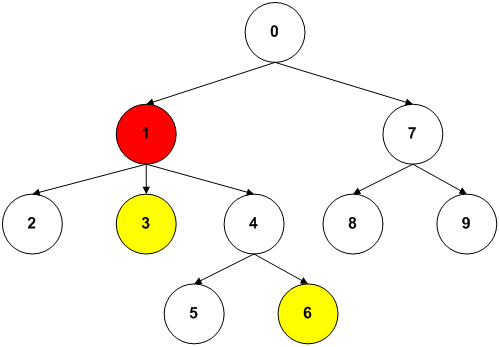
\includegraphics[scale = 0.5]{img/lca1.png}
    \caption{LCA(3,6) = 1}
\end{figure}

 \bigskip
 Note that a node $v$ is considered an ancestor of itself, so LCA(u, v) can also be one of the two.
 The algorithm that we use is offline, meaning that it computes a solution only if we know
 all queries beforehand. Let's now see how it works. 
 
 \medskip
 The algorithm answers all queries
 with a single DFS visit. A query (u, v) is answered at node u, if v has already been visited
 (or vice versa). Let's say we are at node u and want to find LCA(u, v). The answer is either v, or the lowest node among
the ancestors of v that is also an ancestor of u. To each ancestor $a$  of $v$, we assign a set
that contains $a$ itself and all the subtrees with roots in the set of its other children
that are not in the path to $v$. The set that contains u is the answer to our query. The main task is maintaining
efficiently all these sets, and for this purpose we use union find. We also use an auxiliary vector \emph{ancestor} that
will store the real representative of each set \cite{cp}.

After processing all the children of a node u we answer all the
queries(u, v), if v has already been visited. This will be ancestor[\emph{find(u)}]. The full implementation
is shown in Listing \ref{lca}.

\paragraph{Time complexity.} Let's say we have n nodes in the tree and m queries.
The DFS runs in $O(n)$ time. For each of the n nodes we do a find operation and a union operation. Together
with the n makeSet this takes $O(n\alpha(n))$ amortized time.
The total time complexity is: 
$$O(n\alpha(n) + m)$$

\paragraph{Space complexity.} $O(n)$

\lstinputlisting[caption = offline LCA, label=lca]{code/offlineLCA.cpp}
\subsection{Job Sequencing}
\emph{There is a list of $n$ jobs, where each job has a deadline $d$ and a profit $p$ if the job
is completed before the deadline. Find the sub list of jobs that maximizes the total profit, given
that only one job can be scheduled at a certain moment and completing it takes 1 unit of time.}
\begin{figure}[h!]
    \centering
    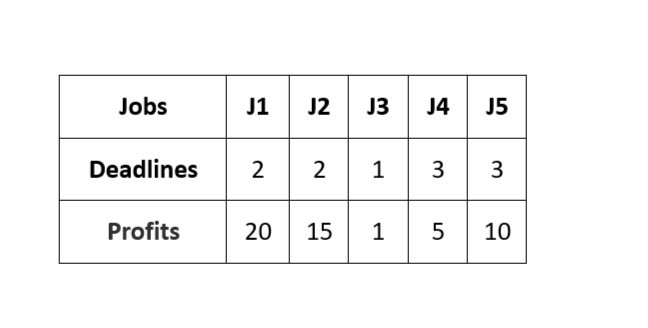
\includegraphics[scale=0.5]{img/jobs.jpeg}
    \caption{A list of jobs with their profit and deadline}
\end{figure}

\bigskip
A greedy solution \cite{key} sorts the list of jobs by decreasing profit and tries to assign each job to the greatest available slot before the deadline, ignoring it if no slots
are found. This algorithm runs in $O(n^2)$.

\medskip

Lets see now a solution that makes use of UnionFind properties. We start by observing that the crucial aspect,
is to keep track of the greatest time slot available for a given job. We do this using disjoint sets. The  representative of a set
is the latest free slot for each job in the set. If a job j is in set 0 it means that no slots can be assigned to it. Finding the representative
of the set corresponds to the \emph{find} operation of UnionFind. When we assign a time slot t
we merge the set t with the set that contains t-1 so that future queries for time slot t will return the latest time slot that is before t. Let's now describe the algorithm in full.

\medskip

The first step is sorting the jobs in decreasing order of their profit. After that, we find the maximum deadline $m$ and create $m+1$ sets, representing the available time slots.
 Now we scan the list  of jobs and, for each job j,
we do the following:\begin{enumerate}
    \item find the latest available slot t
    \item if $t \neq 0$, assign it to the current job and
    execute \emph{union(t-1, t)}
    \item otherwise, skip this job.
\end{enumerate}
If a job is assigned to slot t, it gets executed from $t-1$ to $t$. Assigning a job to slot 0 means that it is ignored.
\paragraph{Time complexity.} Sorting the jobs takes $O(n \log n)$.
A find can take at most $O(\log n)$ and so, the total time complexity is still $O(n\log n)$.
\paragraph{Space complexity.} $O(m)$, where m is the maximum deadline.
\lstinputlisting[caption=Job sequencing, label=jbseq]{code/job_sequencing.cpp}
\bibliographystyle{unsrt}
\bibliography{bib}
\end{document}
